\documentclass[border=10pt]{standalone}
\usepackage{tikz}
\usepackage{pgfplots}
\pgfplotsset{compat=1.18}

\begin{document}

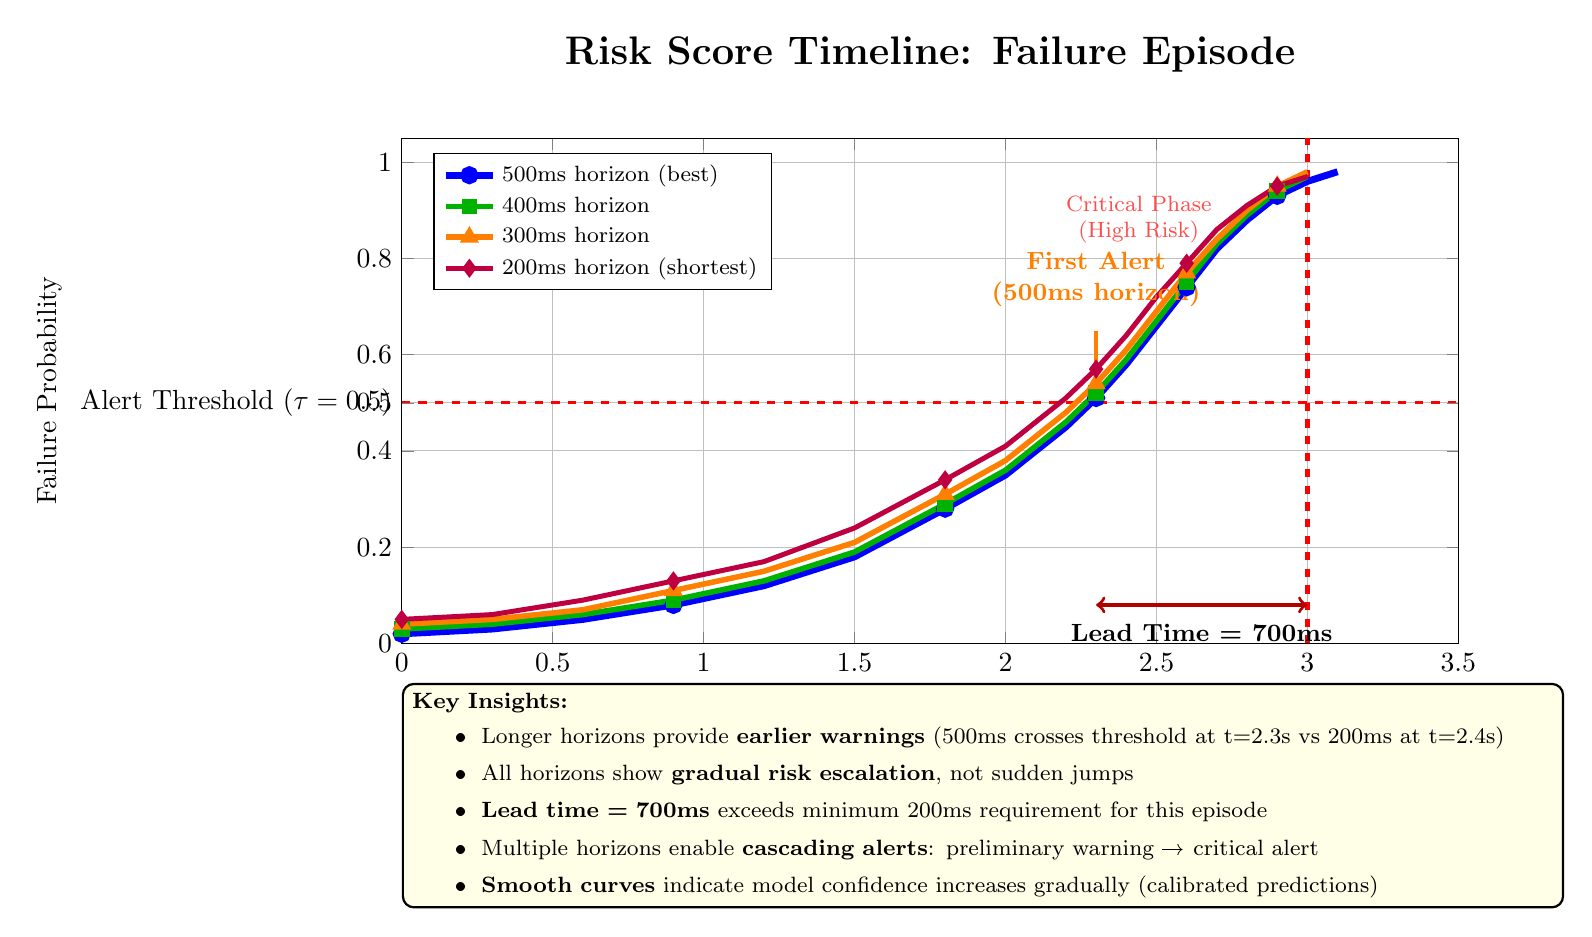
\begin{tikzpicture}
\begin{axis}[
    width=15cm,
    height=8cm,
    xlabel={Time (s)},
    ylabel={Failure Probability},
    legend pos=north west,
    legend style={font=\footnotesize, cells={anchor=west}},
    grid=major,
    xmin=0, xmax=3.5,
    ymin=0, ymax=1.05,
    ytick={0, 0.2, 0.4, 0.5, 0.6, 0.8, 1.0},
    extra y ticks={0.5},
    extra y tick style={grid=major, grid style={red, dashed, line width=1.2pt}},
    extra y tick labels={Alert Threshold ($\tau=0.5$)},
    title={\Large \textbf{Risk Score Timeline: Failure Episode}},
    title style={yshift=0.5cm}
]

% Actual failure at t=3.0s
\draw[red, very thick, dashed, line width=2pt] (axis cs:3.0,0) -- (axis cs:3.0,1.05);
\node[anchor=south, color=red, font=\bfseries\large, rotate=0] at (axis cs:3.0,1.08) {Actual Failure};

% 500ms horizon prediction (primary)
\addplot[color=blue, line width=2.5pt, mark=*, mark size=2pt, mark repeat=3] coordinates {
    (0.0, 0.02) (0.3, 0.03) (0.6, 0.05) (0.9, 0.08)
    (1.2, 0.12) (1.5, 0.18) (1.8, 0.28) (2.0, 0.35)
    (2.2, 0.45) (2.3, 0.51) (2.4, 0.58) (2.5, 0.66)
    (2.6, 0.74) (2.7, 0.82) (2.8, 0.88) (2.9, 0.93)
    (3.0, 0.96) (3.1, 0.98)
};

% 400ms horizon prediction
\addplot[color=green!70!black, line width=2pt, mark=square*, mark size=1.8pt, mark repeat=3] coordinates {
    (0.0, 0.03) (0.3, 0.04) (0.6, 0.06) (0.9, 0.09)
    (1.2, 0.13) (1.5, 0.19) (1.8, 0.29) (2.0, 0.36)
    (2.2, 0.46) (2.3, 0.52) (2.4, 0.59) (2.5, 0.67)
    (2.6, 0.75) (2.7, 0.83) (2.8, 0.89) (2.9, 0.94)
    (3.0, 0.97)
};

% 300ms horizon prediction
\addplot[color=orange, line width=2pt, mark=triangle*, mark size=2pt, mark repeat=3] coordinates {
    (0.0, 0.04) (0.3, 0.05) (0.6, 0.07) (0.9, 0.11)
    (1.2, 0.15) (1.5, 0.21) (1.8, 0.31) (2.0, 0.38)
    (2.2, 0.48) (2.3, 0.54) (2.4, 0.61) (2.5, 0.69)
    (2.6, 0.77) (2.7, 0.84) (2.8, 0.90) (2.9, 0.95)
    (3.0, 0.98)
};

% 200ms horizon prediction
\addplot[color=purple, line width=1.8pt, mark=diamond*, mark size=2pt, mark repeat=3] coordinates {
    (0.0, 0.05) (0.3, 0.06) (0.6, 0.09) (0.9, 0.13)
    (1.2, 0.17) (1.5, 0.24) (1.8, 0.34) (2.0, 0.41)
    (2.2, 0.51) (2.3, 0.57) (2.4, 0.64) (2.5, 0.72)
    (2.6, 0.79) (2.7, 0.86) (2.8, 0.91) (2.9, 0.95)
    (3.0, 0.97)
};

% First alert annotation (500ms horizon crosses threshold)
\draw[orange, very thick, ->] (axis cs:2.3, 0.65) -- (axis cs:2.3, 0.51);
\node[anchor=south, color=orange, font=\small\bfseries, text width=3.5cm, align=center]
     at (axis cs:2.3, 0.68) {First Alert\\(500ms horizon)};

% Lead time annotation
\draw[<->, very thick, color=red!70!black] (axis cs:2.3, 0.08) -- (axis cs:3.0, 0.08);
\node[anchor=north, font=\small\bfseries] at (axis cs:2.65, 0.06) {Lead Time = 700ms};

% Early phase (safe)
\node[anchor=north west, font=\footnotesize, color=black!60, text width=2cm, align=center]
     at (axis cs:0.5, 0.95) {Early Phase\\(Low Risk)};

% Late phase (dangerous)
\node[anchor=north east, font=\footnotesize, color=red!70, text width=2.5cm, align=center]
     at (axis cs:2.8, 0.95) {Critical Phase\\(High Risk)};

\legend{
    500ms horizon (best),
    400ms horizon,
    300ms horizon,
    200ms horizon (shortest)
}

\end{axis}

% Add text box with key insights
\node[anchor=north west, font=\footnotesize, text width=14.5cm, align=left, fill=yellow!10, draw=black, rounded corners, thick]
     at (0, -0.5) {
\textbf{Key Insights:}
\begin{itemize}
    \item Longer horizons provide \textbf{earlier warnings} (500ms crosses threshold at t=2.3s vs 200ms at t=2.4s)
    \item All horizons show \textbf{gradual risk escalation}, not sudden jumps
    \item \textbf{Lead time = 700ms} exceeds minimum 200ms requirement for this episode
    \item Multiple horizons enable \textbf{cascading alerts}: preliminary warning → critical alert
    \item \textbf{Smooth curves} indicate model confidence increases gradually (calibrated predictions)
\end{itemize}
};

\end{tikzpicture}

\end{document}
